\section{Successive Trajectories}
The first step in accomplishing the task would be to raise the pendulum high enough that it would be able to pass through the obstacles. It would be possible to clear a straight path through the obstacles by raising the pendulum from the starting position of $\theta = \pi$ to a little less than $\theta = \frac{\pi}{2}$. Further, the velocity would ideally achieve zero angular velocity as it reaches its target angle. This idea is presented in \autoref{fig:firstTask}, without restricting the pendulum to a specific trajectory but rather showing the initial and final conditions.

\begin{figure}[H]
  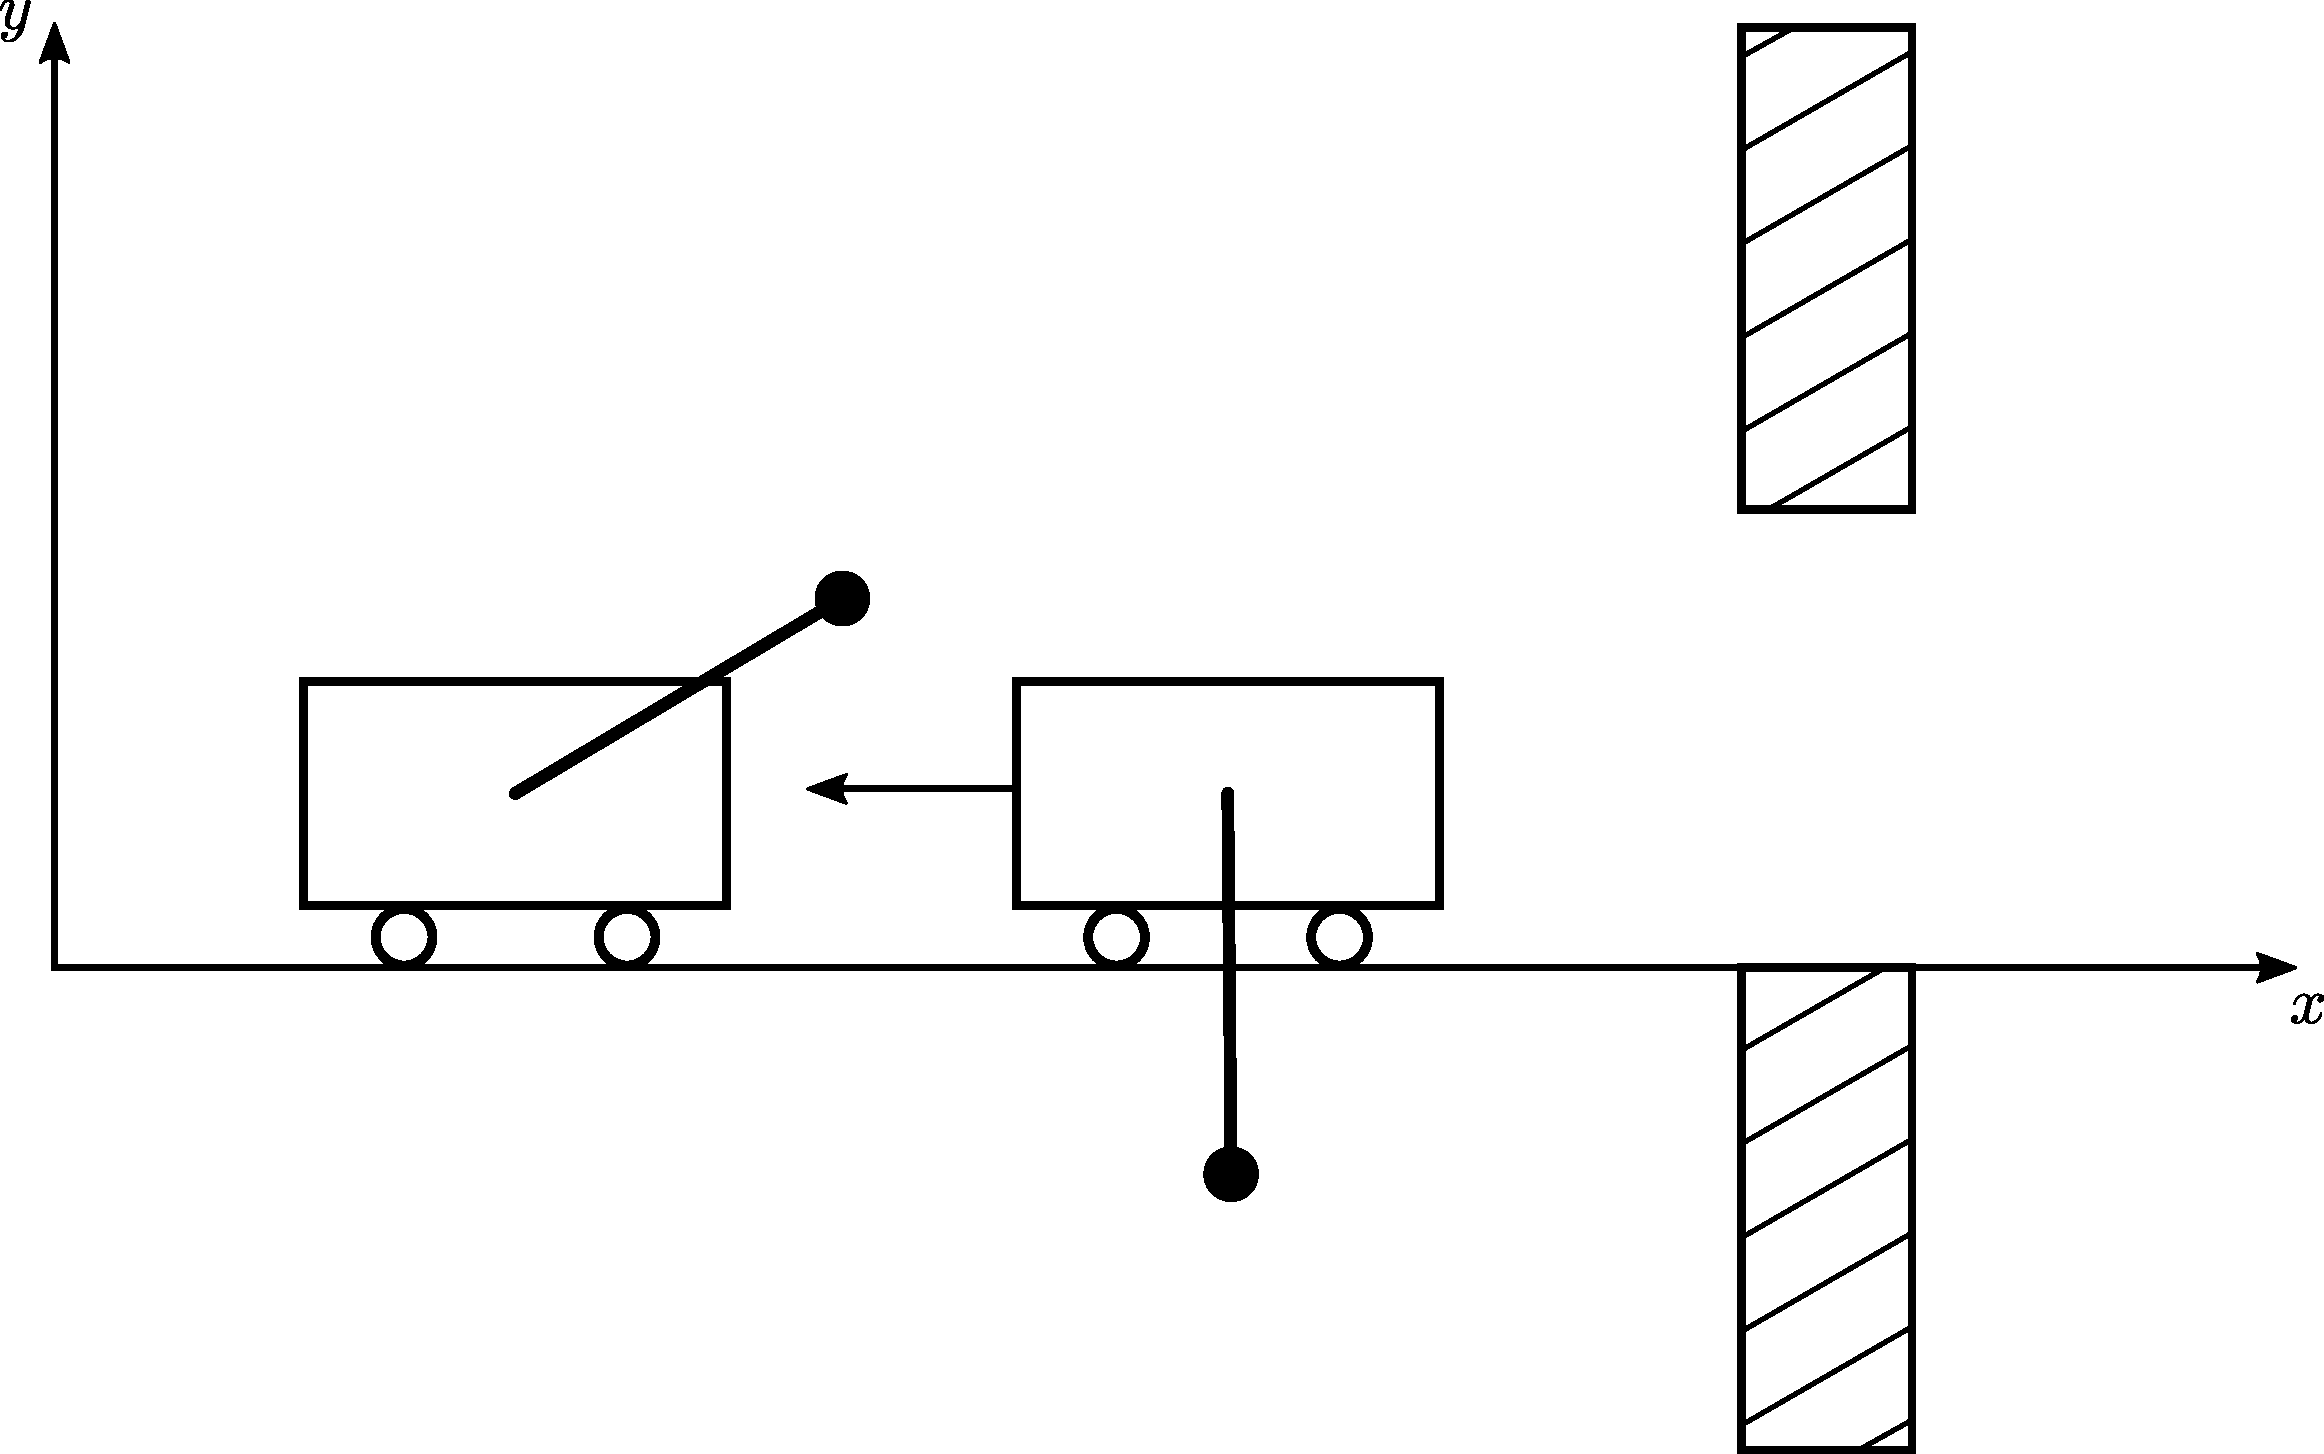
\includegraphics[width=.5\textwidth]{figures/firstTask}
  \caption{The first task is to find a trajectory which raises the pendulum to a position where it is clear of the obstacles in the horizontal direction. Further, to maintain clearance, the angular velocity should hit zero as the target angle is achieved.}
  \label{fig:firstTask}
\end{figure}

The phase portrait in \autoref{fig:phasePortrait}, showing the natural theta-dynamics, it is possible to get an idea of how the pendulum moves. The starting position would be the right-most equilibrium of the phase portrait. If this task should be achieved without external force, the pendulum would have to be initialized in the orbit containing the desired final values. However, by exerting a force on the cart it is possible to shift the theta-dynamics. This is further investigated in the following section.

Assuming that the pendulum was raised above $\frac{\pi}{2}$ while briefly achieving zero angular velocity, the next task would be to maintain zero angular velocity while moving the cart, passing the pendulum through the obstacles, see \autoref{fig:secondTask}.

\begin{figure}[H]
  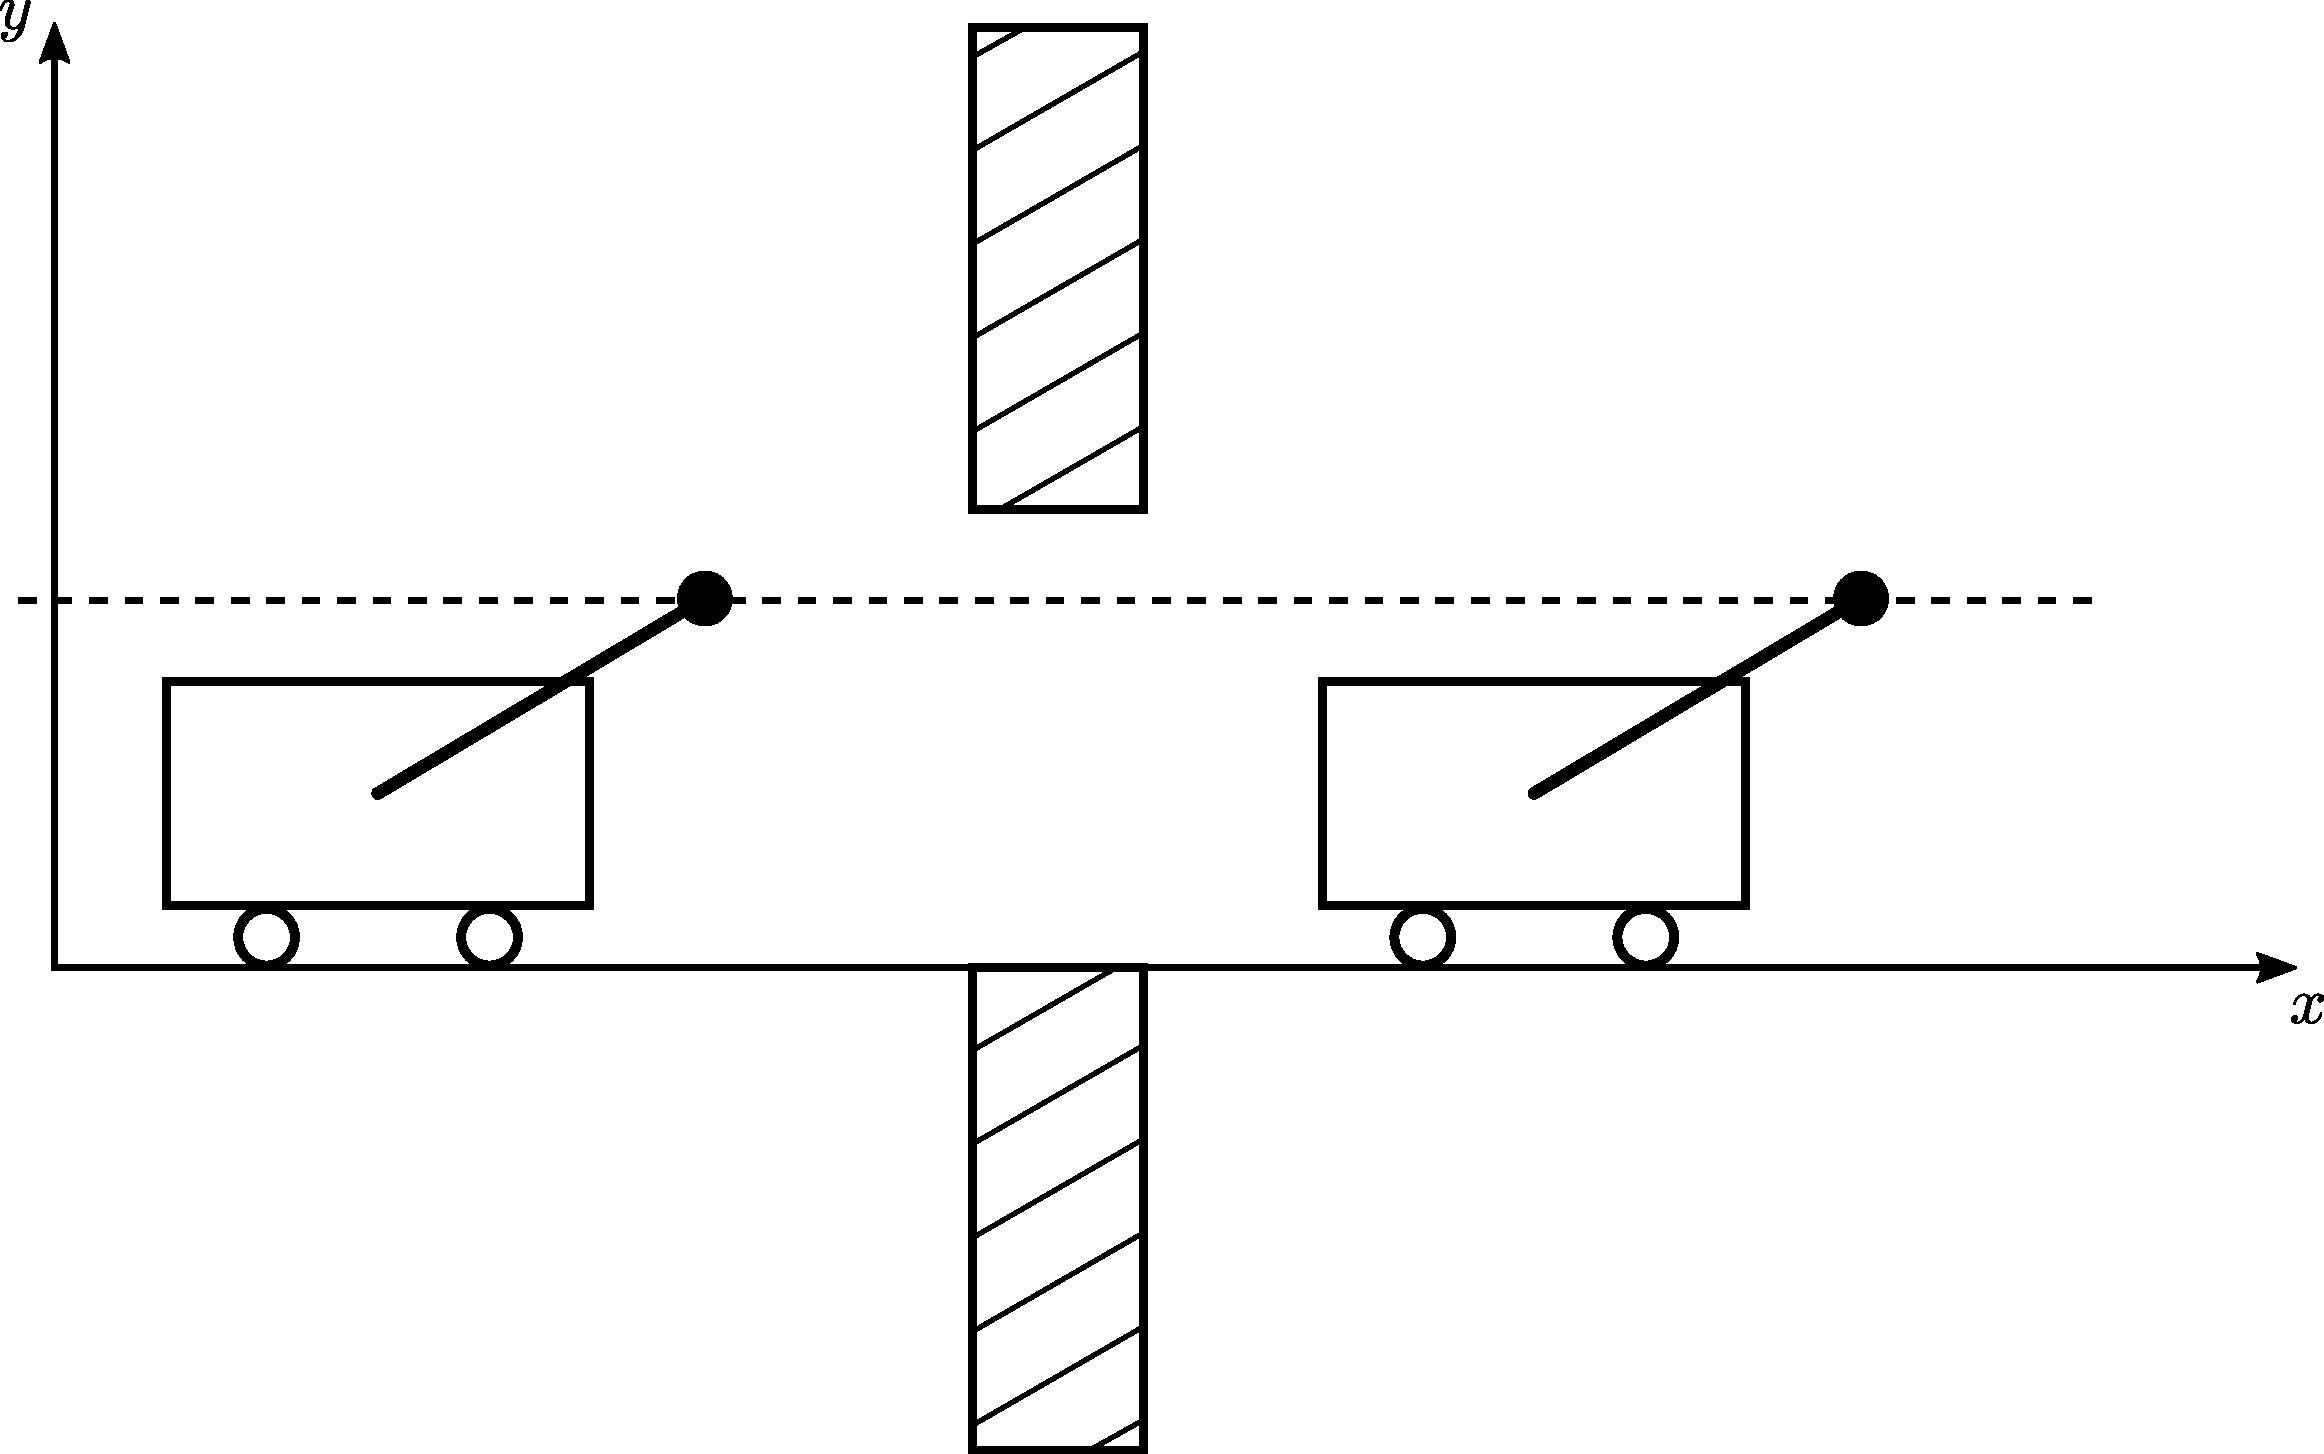
\includegraphics[width=.5\textwidth]{figures/secondTask}
  \caption{The second task is to find a trajectory which keeps the angle and angular velocity at zero as the pendulum is moved with the cart through the obstacles. This can be seen as a virtual constraint where the pendulum is mass is constrained to the dotted line.}
  \label{fig:secondTask}
\end{figure}

Ideally this trajectory is a straight horizontal line. This can be seen as a virtual constraint that forces the angle and the angular velocity to stay unchanged. The result will be significantly reduced dynamics, which can be used to directly achieve the desired trajectory.

Finally it is necessary to recover the system on the other side of the obstacles. It is found that this can be achieved, to some extend, by reversing the first trajectory.